\documentclass[11pt,a4paper]{article}
\usepackage[T1]{fontenc}
\usepackage{lmodern}
\usepackage{a4wide}
\usepackage[dvips]{graphicx}
\usepackage{float}

\usepackage[
pdfauthor={ACE Projekt Team},
pdftitle={Evaluation Algorithms},
pdfcreator={pdftex},
]{hyperref}

\usepackage{sectsty}
\allsectionsfont{\sffamily}

\usepackage{fancyheadings} 
\pagestyle{fancy} 
\lhead{\textsf{\textbf{ACE} \\ \small{a collaborative editor}}}
\chead{}
\rhead{
\includegraphics[height=0.875cm,width=3cm]{../../images/logo_BFH.eps}}
\lfoot{}
\cfoot{\textsf{\thepage}}
\rfoot{}
\setlength{\headrulewidth}{0.6pt}
\setlength{\footrulewidth}{0.6pt}
\setlength{\topmargin}{-50pt}
\addtolength{\headheight}{50pt}

\usepackage{colortbl}

\newcommand{\headercol}[2]{\multicolumn{1}{|>{\bfseries\columncolor[gray]{0.82}}p{#1}|}{\textsf{#2}}}
\newcommand{\ace}[0]{\emph{ACE }}



\begin{document}
\setlength{\parindent}{0pt}

\newtheorem{defn}{Definition}

\bibliographystyle{plain}

\begin{titlepage}
\thispagestyle{empty}
  \includegraphics[height=1.5in]{../../images/pix.eps}

  \begin{center}

    {\fontsize{40}{45} \textbf{\textsf{ACE}}} \\
    \textsf{a collaborative editor} \\
        
    \vspace{36pt}
        
    {\huge{\textbf{\textsf{Report Evaluation Network}}}} \\

    \vspace{36pt}

	\textsf{Berne University of Applied Sciences} \\
    \textsf{School of Engineering and Information Technology} \\
    
  \end{center}

  \vfill
  
  \begin{tabular}{ll}
   \hline

   \\

   \multicolumn{1}{>{\bfseries}p{1.5in}}{\textsf{Date:}} &
   \multicolumn{1}{>{}p{4.3in}}{\textsf{14.06.2005}}          \\
   
   \\
   
   \multicolumn{1}{>{\bfseries}p{1.5in}}{\textsf{Version:}}     &   
   \multicolumn{1}{>{}p{4.3in}}{\textsf{0.6}}                 \\

   \\
   
   \multicolumn{1}{>{\bfseries}p{1.5in}}{\textsf{Projectteam:}}                 &
   \multicolumn{1}{>{}p{4.3in}}{\textsf{Mark Bigler (biglm2@hta-bi.bfh.ch)}}  \\
   \multicolumn{1}{>{\bfseries}p{1.5in}}{}                                      &
   \multicolumn{1}{>{}p{4.3in}}{\textsf{Simon R�ss (rasss@hta-bi.bfh.ch)}}    \\
   \multicolumn{1}{>{\bfseries}p{1.5in}}{}                                      &
   \multicolumn{1}{>{}p{4.3in}}{\textsf{Lukas Zbinden (zbinl@hta-bi.bfh.ch)}} \\   
   
   \\
   
   \multicolumn{1}{>{\bfseries}p{1.5in}}{\textsf{Receivers:}}                       &
   \multicolumn{1}{>{}p{4.3in}}{\textsf{Jean-Paul Dubois (doj@hta-bi.bfh.ch)}}       \\
   \multicolumn{1}{>{\bfseries}p{1.5in}}{}                                          &
   \multicolumn{1}{>{}p{4.3in}}{\textsf{Claude Fuhrer (frc@hta-bi.bfh.ch)}}       \\

   \\
   
   \multicolumn{1}{>{\bfseries}p{1.5in}}{\textsf{Location:}}               &   
   \multicolumn{1}{>{}p{4.3in}}{\textsf{Subversion Repository}} \\

   \\  
   
   \hline
  \end{tabular}

\end{titlepage}

\newpage

\tableofcontents
\newpage
\listoftables
\listoffigures
\newpage


\section*{Versionskontrolle}

\begin{table}[!h]
 \begin{tabular}{|l|l|l|l|}
  \hline
  \headercol{0.6in}{Version}         & 
  \headercol{0.8in}{Datum}           &
  \headercol{1.2in}{Verantwortlich}  & 
  \headercol{2.8in}{Bemerkungen}     \\
  \hline
  0.1         & 15.03.2005  & zbinl           &  Erste Version \\
  0.2         & 16.03.2005  & Projektteam     &  �berarbeitung \\
  0.3         & 05.04.2005  & Projektteam     &  �berarbeitung vor Abgabe \\
  \hline
 \end{tabular}
 \caption{Versionskontrolle}
 \label{Versionskontrolle}
\end{table}

\begin{table}[!h]
 \begin{tabular}{|l|l|l|l|l|}
  \hline
  \headercol{0.9in}{}            & 
  \headercol{0.9in}{Stelle}      & 
  \headercol{0.8in}{Datum}       & 
  \headercol{0.6in}{Visum}       & 
  \headercol{2.0in}{Bemerkungen} \\
  \hline
  \textbf{Freigegeben}   & Projektteam &       &       &             \\
  \hline
  \textbf{Genehmigt}     &             &       &       &             \\
  \hline
 \end{tabular}
 \caption{Pr�fung/Genehmigung}
 \label{Pr�fung/Genehmigung}
\end{table}

\newpage


\section{Introduction}
The purpose of this report is to show usability requirements a user-friendly collaborative editor must have. The most usefull functions will be discussed in the following chapters. There existing also prototypes for some of these functions to ensure the realizability with JAVA text components.

\section{Usability}
Basicaly each user must be distinguishable from all the other users. To do that with different colors is probably one of the best solution. For example the red user has a dark red colored cursor, a light red color to highlight the text he changed and a red border around the text he selected. The users are listed with their colors in a separate window, so all participants can quite easy see which part in the multi-colored document belongs to which user. See \cite{usability} for more information about usability in groupware systems.

\subsection{Main View}
The main view is the users workspace where he can change the document or observe the other users. Important is to keep the main view as simple as possible. This means that it should not be overloaded with a lot of buttons, status labels, etc. because new users will loose their orientation.
\begin{figure}[H]
\centering
\frame{

\includegraphics[height=3cm,width=5cm]{../../images/gui/gui_main_view.eps}
}
\caption{Main View}
\end{figure}

\subsection{Multiple Cursors and Telepointers}
To display the cursors of the other participants is a very usefull feature for observing their changes. This additional cursors must be clearly distinguishable and assigned to a user. Coloring all cursors with the user color (e.g. the green users cursor is painted in dark green) will be the most comfortable way to realize that. Moreover, this cursors should have another form than the standard cursor.

As described above for multiple cursors, it will be user friendly to display the content of the document in different colors too. On this way all participants knows which part is from which user.
\begin{figure}[H]
\centering
\frame{
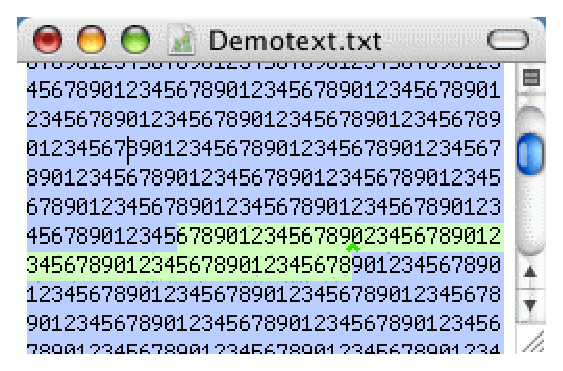
\includegraphics[height=3cm,width=5cm]{../../images/gui/gui_hlight_and_cursor.eps}
}
\caption{Multiple Cursors and Highlighted Text}
\end{figure}
The other users mouse cursors are called telepointers. With this telepointers it is possible to show or explain something in the document. It should be possible to activate/deactivate this telepointers because a lot of different cursors and telepointers can be confusing to the users.
\begin{figure}[H]
\centering
\frame{
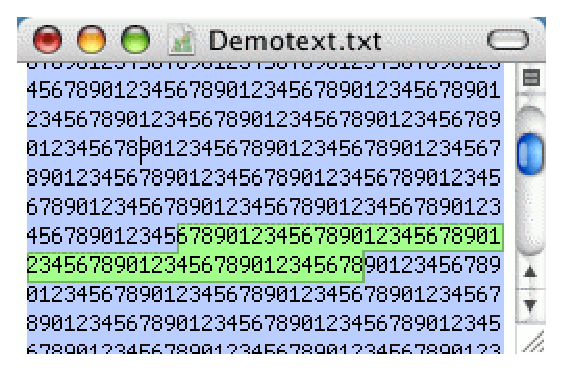
\includegraphics[height=3cm,width=5cm]{../../images/gui/gui_selection.eps}
}
\caption{Text-selection}
\label{Text-selection}
\end{figure}
The picture \ref{Text-selection} shows a possibility to represent selected text of another participant (in this case from the participant associated with the green color).

\subsection{Multi-user Scrollbar}
The aim of multi-user scrollbars is to give a coarse overview of all cursor positions in the document. A user will see his own position by a normal scrollbar and in addition a little colored symbol for the position of each other user.
\begin{figure}[H]
\centering
\frame{
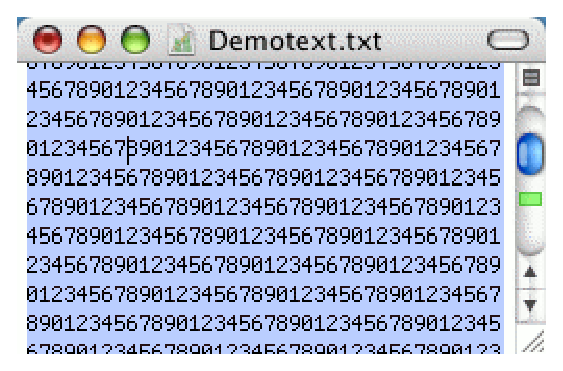
\includegraphics[height=3cm,width=5cm]{../../images/gui/gui_scrollbar.eps}
}
\caption{Multi-user Scrollbar}
\end{figure}

\subsection{Teleport and Split View}
- teleport -> easy showing with shortcut

- splitview -> permanent splitscreen

\subsection{Document and User Handling}
- share documents

- browser shared documents

- invite user / join document

- security and access management


\section{Prototypes}
\subsection{CustomPaint}
\paragraph{Purpose:}
\paragraph{Description:}
\paragraph{Notes:}

\subsection{CustomView}
\paragraph{Purpose:}
\paragraph{Description:}
\paragraph{Notes:}

\subsection{CustomDocument}
\paragraph{Purpose:}
- catch keyborad inputs
\paragraph{Description:}
\paragraph{Notes:}



\section{Other}
\subsection{Undo / Redo}
TODO: describe undo / redo

\subsection{Global Textcomponent Interface}
TODO: describe global interface

\subsection{Distribute Document Changes}
TODO: describe doc changes



\newpage
\appendix
\section{ Appendix }
code fragments


\newpage
\bibliography{ace}

\end{document}
